\documentclass[11pt, xcolor={dvipsnames}, hyperref={colorlinks, allcolors=Blue}]{beamer}


% Packages
\usepackage{graphicx}
\usepackage{caption, subcaption}
\usepackage{tikz}
\usepackage{amsmath, amsfonts, amssymb}
\usepackage{booktabs}
\usepackage{apacite}
\usepackage{multirow}
\usepackage{doi}
\usepackage{textpos}
\usepackage{lipsum}
\usepackage{amsfonts, amsmath}
\usepackage{wrapfig}
\usepackage{animate}
\usepackage{cleveref}


\renewcommand\doiprefix{}


\usepackage{tikz}
\usetikzlibrary{shapes, fit}





%%%%%%%%%%%%%%%%%%%%%%%%%%%%%%%%%%%%%%%%%%%%%%
% Custom commands
\newcommand\bc[1]{{\usebeamercolor[fg]{frametitle} {\textbf{#1}}}} % bold and color
\newcommand{\into}{\rightarrow}



%%%%%%%%%%%%%%%%%%%%%%%%%%%%%%%%%%%%%%%%%%%%%%
% Set Theme
\usetheme{Boadilla}
\usecolortheme{rose}

%%%%%%%%%%%%%%%%%%%%%%%%%%%%%%%%%%%%%%%%%%%%%%
% Make citation font tiny
\renewcommand{\bibliographytypesize}{\tiny}

%%%%%%%%%%%%%%%%%%%%%%%%%%%%%%%%%%%%%%%%%%%%%%
% Fonts
\usefonttheme{serif} % Serif font
\setbeamertemplate{enumerate items}[default] % Don't use bullets in enumerate.

%%%%%%%%%%%%%%%%%%%%%%%%%%%%%%%%%%%%%%%%%%%%%%%
% Remove navigation bar
\setbeamertemplate{navigation symbols}{}
%%%%%%%%%%%%%%%%%%%%%%%%%%%%%%%%%%%%%%%%%%%%%%


% Frontmatter
\title[ECON 8000 -  Lecture 3]{Lecture 3: Linear Algebra I}
\author[University of Queensland]{Robert Garrard}
\date[\today]{} 


%%%%%%%%%%%%%%%%%%%%%%%%%%%%%%%

% Common commands

% Sets
\newcommand{\R}{\mathbb{R}}
\newcommand{\N}{\mathbb{N}}
\newcommand{\Z}{\mathbb{Z}}
\newcommand{\Q}{\mathbb{Q}}
\renewcommand{\P}{\mathbb{P}}
\newcommand{\E}{\mathbb{E}}

% Symbols
\renewcommand{\epsilon}{\varepsilon}
\renewcommand{\implies}{\Rightarrow}
\newcommand{\halmos}{\hfill$\blacksquare$}

% Vector notation
\renewcommand{\b}{\mathbf{b}}
\newcommand{\x}{\mathbf{x}}
\newcommand{\y}{\mathbf{y}}
\newcommand{\z}{\mathbf{z}}
\renewcommand{\v}{\mathbf{v}}



%%%%%%%%%%%%%%%%%%%%%%%%%%%%%%%%

% Tikz
\usetikzlibrary{arrows,shapes,trees, positioning}

%%%%%%%%%%%%%%%%%%%%%%%%%%%%%%

\newcounter{Lecture}
\addtocounter{Lecture}{3}

\newcounter{exercise}
\newenvironment{exercise}[1][]{\refstepcounter{exercise}\par\medskip
   \noindent {\bc{Exercise}~\bc{\theLecture.\theexercise} #1}}{\medskip}

\begin{document}

\begin{frame}
\titlepage


%\begin{picture}(0,0)
%\put(35,-50){\hbox{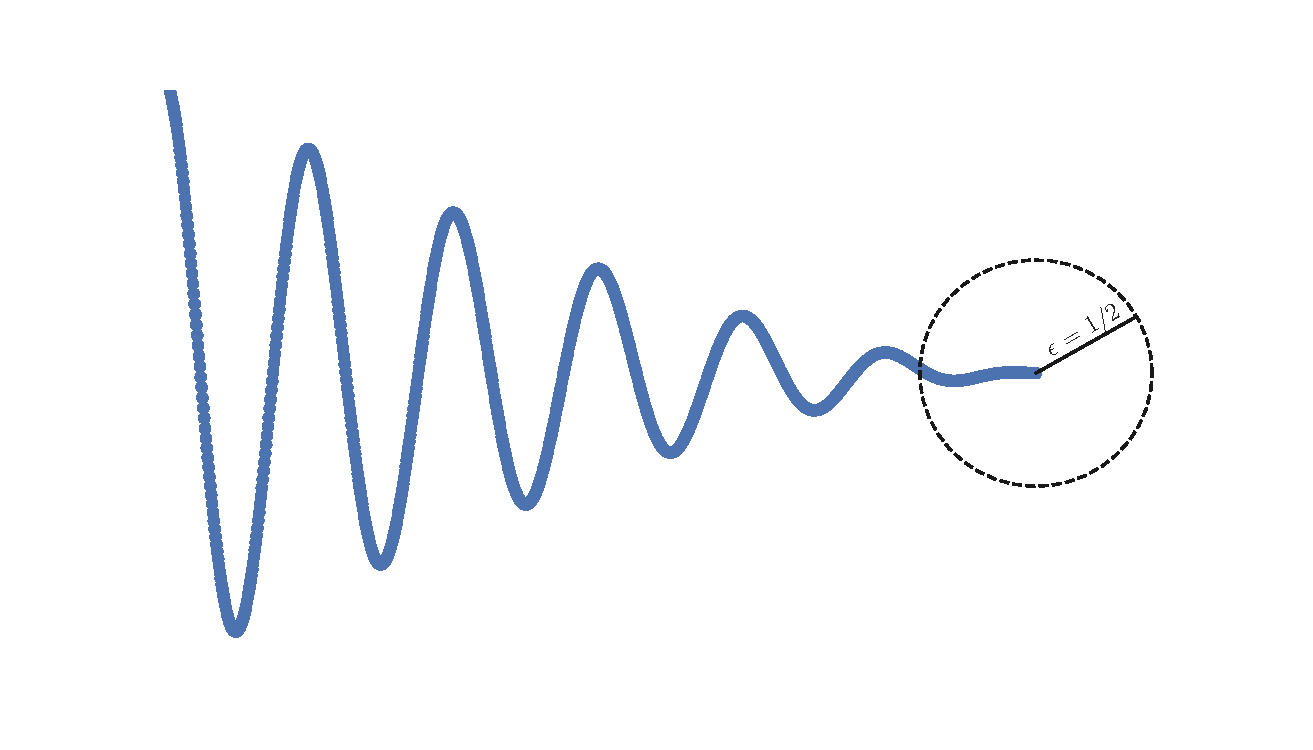
\includegraphics[width=0.8\textwidth, trim={0cm, 1cm, 0cm, 1cm}, clip]{convergence.pdf}}}
%\end{picture}

\end{frame}
%%%%%%%%%%%%%%%%%%%%%%%%%%%%%

\begin{frame}{Systems of Linear Equations}

A \bc{linear} equation in $n$ variables is one in which the highest order of a variable is unity. We're often concerned with solving a set of $m$ linear equations in $n$ variables \emph{simultaneously}. \bigskip


\begin{center}
\begin{tabular}{c c c c c c c c c}
$a_{11}x_{11}$   &+&   $a_{12}x_{12}$      &+&    $\cdots$    &+&    $a_{1n}x_{1n}$   &=& $b_1$\\
$a_{21}x_{21}$   &+&   $a_{22}x_{22}$      &+ &   $\cdots$    &+&    $a_{2n}x_{2n}$   &=& $b_2$\\
$a_{31}x_{31}$   &+&   $a_{32}x_{32}$      &+&    $\cdots$    &+&    $a_{3n}x_{3n}$   &=& $b_3$\\
$\vdots$               &+&        $\vdots$                &+&    $\cdots$    &+&    $\vdots$               &=&  $\vdots$\\
$a_{m1}x_{m1}$  &+&   $a_{m2}x_{m2}$   &+&    $\cdots$    &+&    $a_{mn}x_{mn}$ &=& $b_m$
\end{tabular}
\end{center}

\end{frame}

%%%%%%%%%%%%%%%%%%%%%%%%%%%

\begin{frame}{Systems of Linear Equations}

\noindent
Subscripts are ordered by row then column. That is, $x_{24}$ denotes the second equation and fourth variable. \bigskip

It's convenient to write this system in \bc{augmented matrix} form, where we drop superfluous objects.\bigskip

\[
\left (
\begin{array}{cccc|c}
a_{11} & a_{12} & \cdots & a_{1n} & b_1\\
a_{21} & a_{22} & \cdots & a_{2n} & b_2\\
\vdots & \vdots & \cdots & \vdots & \vdots\\
a_{m1} & a_{m2} & \cdots & a_{mn} & b_m
\end{array}
\right )
\]

\end{frame}

%%%%%%%%%%%%%%%%%%%%%%%%%%%

\begin{frame}{Systems of Linear Equations}

An \bc{elementary row operation} on a system of linear equations is one of the following.\bigskip

\begin{enumerate}[1.]
\item Multiplying a row by a non-zero scalar.
\item Adding two rows together.
\item Switching two rows.
\end{enumerate}
\bigskip

\begin{block}{Proposition}
The solution of a system of linear equations is preserved by elementary row operations.
\end{block}

\end{frame}

%%%%%%%%%%%%%%%%%%%%%%%%%%%%

\begin{frame}{Systems of Linear Equations}

\begin{itemize}
\setlength{\itemsep}{5mm}
\item So we can solve a system by reducing it to something simpler using row operations.

\item There are two good candidates for the form of that simplification: row echelon form and reduced row echelon form. 

\item Row echelon form is obtained in fewer row operations which, as you may know from experience, are prone to arithmetic errors when performed by a human. 

\item Reduced row echelon form has the cost of additional row ops, but has the distinct advantage that the solution set is more easily characterised when there are infinitely many solutions.
\end{itemize}

\end{frame}
%%%%%%%%%%%%%%%%%%%%%%%%%%%%

\begin{frame}{Systems of Linear Equations}


 The \bc{pivot} of a non-zero row is its leftmost non-zero element.\footnote{Some texts require that this element be a 1.} \bigskip

A system of linear equations is said to be in \bc{row echelon form} if the pivot of a non-zero row is strictly to the right of the pivot of the row above it.\bigskip

A system is said to be in \bc{reduced row echelon form} if:
\begin{enumerate}
	\item It is in row echelon form.
	\item Each pivot is the only non-zero entry in its column.
	\item Each pivot is a one.
\end{enumerate}
\end{frame}

%%%%%%%%%%%%%%%%%%%%%%%%%%%%

\begin{frame}{Systems of Linear Equations}
\begin{exercise}

Which of the following systems are in row echelon form? For any that aren't, which row operations would you use? 

\[
\left (
\begin{array}{ccc|c}
2 & 0 & 1 & 1\\
0 & 1 & 1 & 0\\
0 & 0 & 0 & 3
\end{array}
\right )
\quad
\left (
\begin{array}{ccc|c}
0 & 0 & 1 & 0\\
0 & 0 & 1 & 0\\
0 & 4 & 0 & 0
\end{array}
\right )
\quad
\left (
\begin{array}{ccc|c}
0 & 0 & 1 & 0\\
0 & 0 & 0 & 1\\
0 & 0 & 0 & 0
\end{array}
\right )
\]
\bigskip

Which of the following systems are in reduced row echelon form? For any that aren't, which row operations would you use? 

\[
\left (
\begin{array}{ccc|c}
1 & 0 & 1 & 1\\
0 & 1 & 1 & 0\\
0 & 0 & 0 & 0
\end{array}
\right )
\quad
\left (
\begin{array}{ccc|c}
1 & 0 & 3 & 0\\
0 & 2 & 1 & 0\\
0 & 0 & 0 & 0
\end{array}
\right )
\quad
\left (
\begin{array}{ccc|c}
1 & 0 & 1 & 2\\
0 & 1 & 0 & 5\\
0 & 0 & 1 & 0
\end{array}
\right )
\]

\end{exercise}
\end{frame}
%%%%%%%%%%%%%%%%%%%%%%%%%%%%
\begin{frame}{Systems of Linear Equations}

If the $i$th column of the reduced row echelon form contains a pivot, we call $x_{i}$ a \bc{basic variable}.\medskip

 If it does not contain a pivot, we call $x_i$ a \bc{free variable}.\bigskip

\begin{exercise}


Place the following systems in reduced row echelon form. State if each variable is basic or free.

\[
\left (
\begin{array}{ccc|c}
2 & 1 & 0 & 1\\
2 & 1 & 1 & 2\\
4 & 3 & 0 & 3
\end{array}
\right )
\quad
\left (
\begin{array}{cccc|c}
1 & 1 & 1 & 1 & 1\\
2 & 4 & 4 & 2 & 1\\
0 & 1 & 2 & 4 & 1
\end{array}
\right )
\]
\end{exercise}
\end{frame}

%%%%%%%%%%%%%%%%%%%%%%%%%%%%
\begin{frame}{Systems of Linear Equations}

The \bc{rank} of a matrix is the number of non-zero rows in its row echelon form.\footnote{While a system does not necessarily have a unique row echelon form, the number of non-zero rows is the same in every row echelon form.}\bigskip

Let $A$ be an $m\times n$ matrix. 

\begin{itemize}
\item If $\text{rank}(A) = \min\{m,n\}$, $A$ is said to be \bc{full rank}. 
\item Otherwise it is \bc{rank deficient}. 
\item A matrix whose rank is $m$ is said to have \bc{full row rank} and whose rank is $n$ is said to have \bc{full column rank}. 
\end{itemize}\bigskip

Now that we can reduce systems to something simpler, how do we go about characterising the solution?


\end{frame}

%%%%%%%%%%%%%%%%%%%%%%%%%%%%
\begin{frame}{Systems of Linear Equations}
\begin{center}
\textbf{Recipe for Solving a System of Linear Equations}
\end{center}

\begin{enumerate}[1.]
\item Use row operations to put the augmented system in reduced row echelon form.
\item Is the last column of the augmented system a pivot column? If yes, there is no solution. If no, proceed.
\item Are there any free variables? If no, read the unique solution off of each row. If yes, proceed.
\item Solve for each basic variable in terms of the free variables and a constant. 
\end{enumerate}


\end{frame}

%%%%%%%%%%%%%%%%%%%%%%%%%%%%
\begin{frame}{Systems of Linear Equations}
\begin{block}{Example}
Solve the following system of equations. 
\[
\left (
\begin{array}{cccc|c}
1 & 0 & 1 & 0 & 1\\
0 & 1 & 2 & 2  & -1\\
0 & 0 & 0 & 0 & 0
\end{array}
\right )
\]
\noindent
System is already in RREF. The last column does not contain a pivot, so there's at least one solution. There are two free variables, $x_3$ and $x_4$, so there are infinitely many solutions. Solving in terms of free variables and constants gives
\begin{align*}
x_1 &= 1 - x_3\\
x_2 &= -1 - 2x_3 -2x_4\\
x_3 &= x_3\\
x_4 &= x_4 \qquad \text{for any } x_3,x_4 \in \R
\end{align*}

\end{block}
\end{frame}

%%%%%%%%%%%%%%%%%%%%%%%%%%
\begin{frame}{Systems of Linear Equations}
\begin{block}{Example}
\begin{align*}
x_1 &= 1 - x_3\\
x_2 &= -1 - 2x_3 -2x_4\\
x_3 &= x_3\\
x_4 &= x_4 \qquad \text{for any } x_3,x_4 \in \R
\end{align*}

Can be written more compactly in vector notation
\[
\begin{pmatrix}
x_1\\x_2\\x_3\\x_4\\
\end{pmatrix}
=
\begin{pmatrix}1\\-1\\0\\0\end{pmatrix}
+
\begin{pmatrix}-1\\-2\\1\\0\end{pmatrix}x_3
+
\begin{pmatrix}0\\-2\\0\\1\end{pmatrix}x_4
\]
We can see that the solution set is a plane in $\R^4$.
\end{block}
\end{frame}

%%%%%%%%%%%%%%%%%%%%%%%%%%

\begin{frame}{Vector Spaces}
A \bc{vector space} is a structure formed by a set $V$ (whose elements are called vectors) together with two operations: addition and scalar multiplication.\bigskip

 We will only be considering scalars to be the set of real numbers, $\R$, but in general they may be any \bc{field}.\bigskip

For $V$ to be a vector space over some field $F$ equipped with the binary operations of vector addition and scalar multiplication, then $\forall \x, \y, \z \in V$, and for all scalars $r, s \in F$, the following conditions must hold:

\end{frame}

\begin{frame}{Vector Spaces}
\begin{block}{Vector space axioms}
\begin{enumerate}
\item \emph{Commutativity of vector addition} \quad $\x + \y = \y + \x$

\item \emph{Associativity of vector addition} \quad $(\x + \y) + \z = \x + (\y + \z)$

\item \emph{Additive identity:} There is a $\mathbf{0}$ s.t \quad $\mathbf{0} + \x = \x $

\item \emph{Additive inverse:} $\forall \x$ there exists a $-\x$ s.t \quad $\x + -\x = \mathbf{0}$

\item \emph{Associativity of scalar multiplication} \quad $r(s\x) = (r s)\x$

\item \emph{Distributivity of scalar sums} \quad $ (r + s) \x = r\x + s\x$

\item \emph{Distributivity of vector sums} \quad $r(\x + \y) = r\x + r\y$

\item \emph{Scalar identity} \quad $1\cdot \x = \x$

\end{enumerate}
\end{block}
\end{frame}
%%%%%%%%%%%%%%%%%%%%%%%%%%

\begin{frame}{Vector Spaces}

\begin{exercise}
Which of the following, if any, constitute a vector space?
\begin{enumerate}[1.]
\item $(x_{1}, \dots, x_{n}) \in \R^{n}$ with componentwise addition.
\item The set of square matrices under matrix addition.
\item The set of $3 \times 3$ matrices under matrix addition.
\item The set of $3 \times 3$ matrices under matrix multiplication.
\item The set of functions from $\R$ to $\R$ under $(f+g)(x) = f(x) + g(x)$.
\end{enumerate}
\end{exercise}
\end{frame}
%%%%%%%%%%%%%%%%%%%%%%%%%%

\begin{frame}{Vector Spaces}

Let $V$ be a vector space over $\R$ and let $v_1,\dots,v_n$ be vectors in $V$.\bigskip

The vectors $v_1,\dots,v_n$ are \bc{linearly independent} if, for scalars $c_1,\dots,c_n \in \R$, the only solution to the equation
\[c_1v_1 + \dots + c_n v_n = 0\]

is $c_1 = 0, \dots, c_n = 0$.
\bigskip

The vectors $v_1,\dots,v_n$ are \bc{spanning} if for every vector $v\in V$, we can find $c_1, \dots, c_n \in \R$ such that
\[v = c_1 v_1 + \dots + c_n v_n\]
In which case we may write $V = \text{span}\{v_1,\dots,v_n\}$.

\end{frame}


\begin{frame}{Vector Spaces}

The vectors $v_1,\dots,v_n$ form a \bc{basis} for $V$ if they are linearly independent and spanning. \bigskip


A vector space is finite dimensional with dimension $n$ if we can find a vectors $v_1,\dots,v_n \in V$ which form a basis for $V$.\bigskip


\begin{exercise}


Show that $\R^{n}$ is $n$-dimensional.
\end{exercise}


\end{frame}


%%%%%%%%%%%%%%%%%%%%%%%%
\begin{frame}{Subspaces}

A subset $W \subset V$ is called a \bc{subspace} if and only if

\begin{enumerate}[1.]
\item $\mathbf{0} \in W$
\item If $\mathbf{u},\mathbf{v} \in W$ then $\mathbf{u} + \mathbf{v} \in W$
\item If $\mathbf{u} \in W$ then $\alpha\mathbf{u}\in W$ for any scalar $\alpha \in \R$
\end{enumerate}
\bigskip

Let $v_1,\dots,v_n\in V$. The \bc{span} of the list of vectors is
\[\text{span}\{v_1,\dots,v_n\} = \{c_1v_1 +\dots + c_n v_n \ | \ \forall c_1,\dots,c_n \in \R\}\]

Note that the span of a list of vectors forms a subspace. Moreover, the list is a spanning set for that subspace.\\

\end{frame}
%%%%%%%%%%%%%%%%%%%%%%%%
\begin{frame}{Subspaces}

\begin{exercise}


\begin{enumerate}
\setlength{\itemsep}{5mm}
\item What's the difference between a spanning set and a basis?
\item Let $v_1 = [1, 1, 0]^\prime$, $v_2 = [1, 0, 1]^\prime$, $v_3 = [1,1,1]^\prime$. 
	\begin{enumerate}[a)]
	\item Find $\text{span}\{v_1,v_2,v_3\}$. 
	\item Find a basis for the spanning subspace.
	\item What's the dimension of the spanning subspace?
	\end{enumerate}
\item Under what conditions is a plane a subspace of $\R^{3}$?
\end{enumerate}

\end{exercise}


\end{frame}


%%%%%%%%%%%%%%%%%%%%%%%%%%%%%
\begin{frame}{Linear Mappings}

Consider the vector spaces $\R^{m}$ and $\R^{n}$. A function $f:\R^{m}\to\R^{n}$ is a \bc{linear map} if: 
\begin{itemize}
\item $f(x + y) = f(x) + f(y)$ \ $\forall x,y\in V$.
\item $f(\alpha x) = \alpha f(x)$ \ $\forall \alpha \in \R, \ x \in V$.
\end{itemize}
\bigskip

\begin{block}{Proposition}
Let $f:\R^{m}\to\R^{n}$ be a linear map. Further, let the vectors of $\R^{m}$ and $\R^{n}$ be column vectors. Then there exists a matrix $A$ such that
\[f(\v)\ = A\v\]
\end{block}
\bigskip

That is to say that matrices are not just a convenience for solving systems of linear equations, instead they may be thought of as linear functions between vector spaces. 
\end{frame}

%%%%%%%%%%%%%%%%%%%%%%%%%%%%%
\begin{frame}{Linear Mappings}
But if they're functions, do they have analogues of certain interesting structures functions have?\bigskip


Recall that for a function $f:X\to Y$, the \bc{image} of that function is the set
\[\text{im}(f) = \{ y \in Y \ | \ \exists x\in X s.t \ f(x) = y\} \]


Equations like $f(x) = b$ have a solution if and only if $b \in im(f)$.\bigskip

 Furthermore, if the function is \bc{surjective}, meaning the image of the function equals its codomain, then for any $b$ there is a solution to $f(x) = b$. How might this look in the special case of \emph{linear} functions. 

\end{frame}

\begin{frame}{The Column Space}
Consider the function $A\v$ for some arbitrary $\v$. We can decompose it to

\[
\left (
\begin{array}{c c c c}
a_{11} & a_{12} & \cdots & a_{1n}\\
\vdots & \vdots & \cdots & \vdots\\
a_{m1} & a_{m2} & \cdots & a_{mn}
\end{array}
\right)
\left(
\begin{array}{c}v_1 \\ \vdots \\ v_n\end{array}
\right)
\]
\[
=
\left(\begin{array}{c}a_{11}\\\vdots\\a_{m1}\end{array}\right)v_1+\left(\begin{array}{c}a_{12}\\\vdots\\a_{m2}\end{array}\right)v_2 +\cdots+\left(\begin{array}{c}a_{1n}\\\vdots\\a_{mn}\end{array}\right)v_n
\]
\[ = \mathbf{a}_{1}v_1 + \mathbf{a}_{2}v_2 + \cdots + \mathbf{a}_{n}v_n\]
\bigskip

The output of the function is a linear combination of the columns of $A$. So the image of the function must be the subspace spanned by the columns of $A$!
\end{frame}

\begin{frame}{The Column Space}
The \bc{column space} of an $m\times n$ matrix $A$, $\mathrm{Col}(A)$, is the subset of $\R^{n}$ spanned by its columns.\bigskip

\begin{exercise}

Consider the following matrices.
\[ 
\left ( \begin{array}{c c} 1 & 2 \\ 2 & 4\end{array}\right)
\qquad
\left ( \begin{array}{c c} 1 & 2 \\ 0 & 0\end{array} \right)
\]
What do you notice about the relationship between these matrices? Find a basis for the col space of each, what can you conclude?
\end{exercise}


\end{frame}

%%%%%%%%%%%%%%%%%%%%%%%%%%%%%%
\begin{frame}{The Column Space}

\begin{theorem}
The basic columns of $A$ form a basis for $\mathrm{Col}(A)$.

\end{theorem}
\bigskip
While row ops don't preserve the span of the columns, they do preserve any dependence relationship between them.\bigskip

 That is, linearly independent columns will still be linearly independent in a row echelon form. This lets us easily refine a spanning set (the whole set of columns) down to a basis (a minimal spanning set).

\end{frame}

%%%%%%%%%%%%%%%%%%%%%%%%%%%%%%
\begin{frame}{The Column Space}

\begin{theorem}
Let $A$ be an $m \times n$ matrix.
\begin{enumerate}[a)]
\item The system of equations $A\x = \mathbf{b}$ has a solution for a particular $\b\in \R^{m}$ if and only if $\b\in \mathrm{Col}(A)$.
\item The system $A\x = \b$ has a solution for \emph{every} $\b$ if and only if $rank(A) = m$. That is, $A$ has full row rank. 
\item $dim \ \text{Col}(A) = \text{Rank}(A)$.
\end{enumerate}
\end{theorem}

\end{frame}

%%%%%%%%%%%%%%%%%%%%%%%%%%%%%%
\begin{frame}{The Null Space}

Another interesting property functions have is the set of zeros: $\{x \ | \ f(x) = 0\}$.(i.e., the pre-image of 0) \bigskip

Define the \bc{null space} (elsewhere called the \bc{kernel}) of an $m \times n$  matrix $A$, denoted $\text{Null}(A)$, to be the set of vectors that solve $A\x = \mathbf{0}$.\bigskip

\bc{Exercise:} Show that the null space is a subspace of $\R^{n}$.
\end{frame}

%%%%%%%%%%%%%%%%%%%%%%%%%%%%%%
\begin{frame}{Affine Subspaces}

Let $V$ be a subspace of $\R^{n}$ and $\mathbf{c} \in \R^{n}$ be a fixed vector. A set of the form

\[ \{\x \in \R^{n} \ | \ \x = \mathbf{c} + \v \text{ for some } \v \in V\}\]

is called an \bc{affine subspace} of $\R^{n}$.\bigskip

\textbf{Affine subspaces are not subspaces!} (why?)\bigskip

It does preserve linearity, and we say its dimension is the dimension of $V$.
\end{frame}
%%%%%%%%%%%%%%%%%%%%%%%%%%%%%%
\begin{frame}{The Solution Set is an Affine Subspace}

Let $A\x = \b$ be an $m \times n$ system of equations and let $\mathcal{S} = \{\x \in \R^{n} \ | A\x = \b\}$ be the set of solutions to the system.\bigskip

\begin{theorem}
If $\mathcal{S}$ is non-empty, such that there is at least one particular solution, $\x^{*}$, such that $A\x^{*} = \b$. Then $\mathcal{S}$ is the affine subspace

\[\mathcal{S} = \{\x^{*} + \v \ | \ \v \in \text{Null}(A)\}\]
\end{theorem}

Proof (tutorial excercise) 
\end{frame}

%%%%%%%%%%%%%%%%%%%%%%%%%%%%%%

\begin{frame}{The Fundamental Theorem of Linear Algebra}

\begin{theorem}[Rank-Nullity theorem]
Let $A$ be an $m \times n$ matrix. Then
\[ \text{rank}(A) + dim \text{Null}(A) = n\]
\end{theorem}
\bigskip

Recall that $\text{rank}(A) = dim \text{Col}(A)$.\bigskip

The column space tells us whether the equation has a solution.\bigskip

The null space tells us how large the solution set is. 
\end{frame}
%%%%%%%%%%%%%%%%%%%%%%%%%%%%%%

\begin{frame}{Number of solutions to a system of equations}
\begin{itemize}
	\item If $\text{rank}(A) = m$, the number of rows, then $A\x = \b$ has a solution for every $\b$.
	\item If $\text{rank}(A) < m$, then $A\x = \b$ will only have a solution for $b \in \text{Col}(A)$.
	\item If $\text{rank}(A) = n$, the matrix is full column rank, then $\text{Null}(A) = \{\mathbf{0}\}$, and $A\x = \b$ will have \emph{at most} one solution for any $\b$.
	\item If $\text{rank}(A) < n$, then if $A\x = \b$ has a solution, it will have an affine subspace of solutions of dimension $n - \text{rank}(A)$.
\end{itemize}
\end{frame}

%%%%%%%%%%%%%%%%%%%%%%%%%%%%%%

\begin{frame}{Square Matrices and Invertibility}
Let $A$ be an $n \times n$ (square) matrix. \bigskip

Suppose $A$ is full rank, $\text{rank}(A) = n$. 
\begin{itemize}
	\item Since its rank equals the number of rows, $A\x = \b$ has \emph{at least} one solution for every $\b$.
	\item Since its rank equals the number of columns, $A\x = \b$ has \emph{at most} one solution for every $\b$.
	\item Therefore, $A\x = \b$ has a unique solution for every $\b$.
\end{itemize}

\end{frame}
%%%%%%%%%%%%%%%%%%%%%%%%%%%%%%

\begin{frame}{Square Matrices and Invertibility}
So consider the function $f:\R^{n}\to\R^{n}$, $f(\v) = A\v$.\bigskip

\begin{itemize}
	\item if $A\x =\b$ and $A\y = \b$, then it must be that $\x = \y$, since solutions are unique. So $f$ is an injection!
	\item For every $\b \in \R^{n}$ there is an $\x$ such that $f(\x) = \b$, so $f$ is a surjection!
	\item $f$ is a bijection! $f$ must have an inverse function, $f^{-1}:\R^{n}\to\R^{n}$!
\end{itemize} 
\bigskip

\begin{exercise}

Show that $f^{-1}$ must be a linear mapping.

\end{exercise}

\end{frame}

%%%%%%%%%%%%%%%%%%%%%%%%%%%%%%

\begin{frame}{Square Matrices and Invertibility}
If $f^{-1}:\R^{n} \to \R^{n}$ is a linear mapping, it can be represented by a matrix! 

\[ f^{-1}(v) = A^{-1}v\]

This gives us that 

\begin{align*}
&f^{-1}(f(\v)) = A^{-1}A\v = \v\\
& f(f^{-1}(\v)) = A A^{-1} \v = \v
\end{align*}

Which must mean that $A^{-1}A = A A^{-1} = I$.
\end{frame}

%%%%%%%%%%%%%%%%%%%%%%%%%%%%%%

\begin{frame}{The Determinant}

Let $A$ be an $n\times n$ matrix. Let $A_{ij}$ be the $(n-1)\times (n-1)$ submatrix obtained by deleting row $i$ and column $j$ from $A$.\bigskip

 The $(i,j)$th \bc{minor} of $A$ is the scalar
\[M_{ij} = det\left(A_{ij}\right) \]

The $(i,j)$th \bc{cofactor} of $A$ is the scalar 
\[C_{ij} = (-1)^{i+j} M_{ij}\]

The \bc{determinant} of $A$ is given by
\[ det(A) = \sum_{i=1}^{n} a_{1i}C_{1i}\]

Observe that the definition of the determinant is recursive. Computing a determinant requires that we compute the determinants of submatrices. This is resolved by defining the determinant of a scalar to be 
\[\det(a_{ij}) = a_{ij}\]

\end{frame}

%%%%%%%%%%%%%%%%%%%%%%%%%%%%%
\begin{frame}{The Determinant}

\begin{block}{Example}
Compute the determinant of $A = \begin{pmatrix} a & b\\ c & d \end{pmatrix}$

Expand along the top row, find the minors and cofactors.

\begin{align*}
&M_{11} = d&  &M_{12} = c&\\
&C_{11} = (-1)^{2}d = d&  & C_{12} = (-1)^{3}c = -c&
\end{align*}

\[\det(A) = a_{11}C_{11} + a_{12}C_{12} = ad - bc\]

\end{block}

\end{frame}

%%%%%%%%%%%%%%%%%%%%%%%%%%%%%
\begin{frame}{The Determinant}

Let $A$ be an $n \times n$ matrix. 

\begin{theorem}
$A$ is invertible iff $\det(A) \not = 0$.
\end{theorem}
\bigskip

Let the matrix of cofactors be $C$,
\[C =
 \begin{pmatrix}
 c_{1,1} & \dots & c_{1,n}\\ 
\vdots & \ddots & \vdots\\
c_{n,1} & \dots & c_{n,n}
\end{pmatrix}
\]

The \bc{adjugate} (elsewhere called adjoint) of $A$ is 
\[adj(A) = C^{T}\]
\end{frame}

%%%%%%%%%%%%%%%%%%%%%%%%%%%%%

\begin{frame}{The Inverse}
\begin{theorem}
Let $A$ be an invertible matrix. Then
\[A^{-1} = \frac{1}{\det(A)}\, adj(A)\]
\end{theorem}
\end{frame}

\begin{frame}{Learning Outcomes}
You should be able to:
\begin{itemize}
	\item Transform an augmented matrix into row echelon and reduced row echelon form.
	\item Solve a system of equations.
	\item Determine the number of solutions a system of linear equations has given appropriate information.
	\item Apply the axioms of a vector space in proofs.
	\item Apply the definitions of a subspace and the span operator.
	\item Find a basis for the column space of a given matrix.
	\item Calculate the determinant of a matrix of size $2\times2$ and $3\times3$.
\end{itemize}
\end{frame}
\end{document}